
\documentclass{article} % For LaTeX2e
\usepackage{iclr2024_conference,times}

% Optional math commands from https://github.com/goodfeli/dlbook_notation.
%%%%% NEW MATH DEFINITIONS %%%%%

\usepackage{amsmath,amsfonts,bm}

% Mark sections of captions for referring to divisions of figures
\newcommand{\figleft}{{\em (Left)}}
\newcommand{\figcenter}{{\em (Center)}}
\newcommand{\figright}{{\em (Right)}}
\newcommand{\figtop}{{\em (Top)}}
\newcommand{\figbottom}{{\em (Bottom)}}
\newcommand{\captiona}{{\em (a)}}
\newcommand{\captionb}{{\em (b)}}
\newcommand{\captionc}{{\em (c)}}
\newcommand{\captiond}{{\em (d)}}

% Highlight a newly defined term
\newcommand{\newterm}[1]{{\bf #1}}


% Figure reference, lower-case.
\def\figref#1{figure~\ref{#1}}
% Figure reference, capital. For start of sentence
\def\Figref#1{Figure~\ref{#1}}
\def\twofigref#1#2{figures \ref{#1} and \ref{#2}}
\def\quadfigref#1#2#3#4{figures \ref{#1}, \ref{#2}, \ref{#3} and \ref{#4}}
% Section reference, lower-case.
\def\secref#1{section~\ref{#1}}
% Section reference, capital.
\def\Secref#1{Section~\ref{#1}}
% Reference to two sections.
\def\twosecrefs#1#2{sections \ref{#1} and \ref{#2}}
% Reference to three sections.
\def\secrefs#1#2#3{sections \ref{#1}, \ref{#2} and \ref{#3}}
% Reference to an equation, lower-case.
\def\eqref#1{equation~\ref{#1}}
% Reference to an equation, upper case
\def\Eqref#1{Equation~\ref{#1}}
% A raw reference to an equation---avoid using if possible
\def\plaineqref#1{\ref{#1}}
% Reference to a chapter, lower-case.
\def\chapref#1{chapter~\ref{#1}}
% Reference to an equation, upper case.
\def\Chapref#1{Chapter~\ref{#1}}
% Reference to a range of chapters
\def\rangechapref#1#2{chapters\ref{#1}--\ref{#2}}
% Reference to an algorithm, lower-case.
\def\algref#1{algorithm~\ref{#1}}
% Reference to an algorithm, upper case.
\def\Algref#1{Algorithm~\ref{#1}}
\def\twoalgref#1#2{algorithms \ref{#1} and \ref{#2}}
\def\Twoalgref#1#2{Algorithms \ref{#1} and \ref{#2}}
% Reference to a part, lower case
\def\partref#1{part~\ref{#1}}
% Reference to a part, upper case
\def\Partref#1{Part~\ref{#1}}
\def\twopartref#1#2{parts \ref{#1} and \ref{#2}}

\def\ceil#1{\lceil #1 \rceil}
\def\floor#1{\lfloor #1 \rfloor}
\def\1{\bm{1}}
\newcommand{\train}{\mathcal{D}}
\newcommand{\valid}{\mathcal{D_{\mathrm{valid}}}}
\newcommand{\test}{\mathcal{D_{\mathrm{test}}}}

\def\eps{{\epsilon}}


% Random variables
\def\reta{{\textnormal{$\eta$}}}
\def\ra{{\textnormal{a}}}
\def\rb{{\textnormal{b}}}
\def\rc{{\textnormal{c}}}
\def\rd{{\textnormal{d}}}
\def\re{{\textnormal{e}}}
\def\rf{{\textnormal{f}}}
\def\rg{{\textnormal{g}}}
\def\rh{{\textnormal{h}}}
\def\ri{{\textnormal{i}}}
\def\rj{{\textnormal{j}}}
\def\rk{{\textnormal{k}}}
\def\rl{{\textnormal{l}}}
% rm is already a command, just don't name any random variables m
\def\rn{{\textnormal{n}}}
\def\ro{{\textnormal{o}}}
\def\rp{{\textnormal{p}}}
\def\rq{{\textnormal{q}}}
\def\rr{{\textnormal{r}}}
\def\rs{{\textnormal{s}}}
\def\rt{{\textnormal{t}}}
\def\ru{{\textnormal{u}}}
\def\rv{{\textnormal{v}}}
\def\rw{{\textnormal{w}}}
\def\rx{{\textnormal{x}}}
\def\ry{{\textnormal{y}}}
\def\rz{{\textnormal{z}}}

% Random vectors
\def\rvepsilon{{\mathbf{\epsilon}}}
\def\rvtheta{{\mathbf{\theta}}}
\def\rva{{\mathbf{a}}}
\def\rvb{{\mathbf{b}}}
\def\rvc{{\mathbf{c}}}
\def\rvd{{\mathbf{d}}}
\def\rve{{\mathbf{e}}}
\def\rvf{{\mathbf{f}}}
\def\rvg{{\mathbf{g}}}
\def\rvh{{\mathbf{h}}}
\def\rvu{{\mathbf{i}}}
\def\rvj{{\mathbf{j}}}
\def\rvk{{\mathbf{k}}}
\def\rvl{{\mathbf{l}}}
\def\rvm{{\mathbf{m}}}
\def\rvn{{\mathbf{n}}}
\def\rvo{{\mathbf{o}}}
\def\rvp{{\mathbf{p}}}
\def\rvq{{\mathbf{q}}}
\def\rvr{{\mathbf{r}}}
\def\rvs{{\mathbf{s}}}
\def\rvt{{\mathbf{t}}}
\def\rvu{{\mathbf{u}}}
\def\rvv{{\mathbf{v}}}
\def\rvw{{\mathbf{w}}}
\def\rvx{{\mathbf{x}}}
\def\rvy{{\mathbf{y}}}
\def\rvz{{\mathbf{z}}}

% Elements of random vectors
\def\erva{{\textnormal{a}}}
\def\ervb{{\textnormal{b}}}
\def\ervc{{\textnormal{c}}}
\def\ervd{{\textnormal{d}}}
\def\erve{{\textnormal{e}}}
\def\ervf{{\textnormal{f}}}
\def\ervg{{\textnormal{g}}}
\def\ervh{{\textnormal{h}}}
\def\ervi{{\textnormal{i}}}
\def\ervj{{\textnormal{j}}}
\def\ervk{{\textnormal{k}}}
\def\ervl{{\textnormal{l}}}
\def\ervm{{\textnormal{m}}}
\def\ervn{{\textnormal{n}}}
\def\ervo{{\textnormal{o}}}
\def\ervp{{\textnormal{p}}}
\def\ervq{{\textnormal{q}}}
\def\ervr{{\textnormal{r}}}
\def\ervs{{\textnormal{s}}}
\def\ervt{{\textnormal{t}}}
\def\ervu{{\textnormal{u}}}
\def\ervv{{\textnormal{v}}}
\def\ervw{{\textnormal{w}}}
\def\ervx{{\textnormal{x}}}
\def\ervy{{\textnormal{y}}}
\def\ervz{{\textnormal{z}}}

% Random matrices
\def\rmA{{\mathbf{A}}}
\def\rmB{{\mathbf{B}}}
\def\rmC{{\mathbf{C}}}
\def\rmD{{\mathbf{D}}}
\def\rmE{{\mathbf{E}}}
\def\rmF{{\mathbf{F}}}
\def\rmG{{\mathbf{G}}}
\def\rmH{{\mathbf{H}}}
\def\rmI{{\mathbf{I}}}
\def\rmJ{{\mathbf{J}}}
\def\rmK{{\mathbf{K}}}
\def\rmL{{\mathbf{L}}}
\def\rmM{{\mathbf{M}}}
\def\rmN{{\mathbf{N}}}
\def\rmO{{\mathbf{O}}}
\def\rmP{{\mathbf{P}}}
\def\rmQ{{\mathbf{Q}}}
\def\rmR{{\mathbf{R}}}
\def\rmS{{\mathbf{S}}}
\def\rmT{{\mathbf{T}}}
\def\rmU{{\mathbf{U}}}
\def\rmV{{\mathbf{V}}}
\def\rmW{{\mathbf{W}}}
\def\rmX{{\mathbf{X}}}
\def\rmY{{\mathbf{Y}}}
\def\rmZ{{\mathbf{Z}}}

% Elements of random matrices
\def\ermA{{\textnormal{A}}}
\def\ermB{{\textnormal{B}}}
\def\ermC{{\textnormal{C}}}
\def\ermD{{\textnormal{D}}}
\def\ermE{{\textnormal{E}}}
\def\ermF{{\textnormal{F}}}
\def\ermG{{\textnormal{G}}}
\def\ermH{{\textnormal{H}}}
\def\ermI{{\textnormal{I}}}
\def\ermJ{{\textnormal{J}}}
\def\ermK{{\textnormal{K}}}
\def\ermL{{\textnormal{L}}}
\def\ermM{{\textnormal{M}}}
\def\ermN{{\textnormal{N}}}
\def\ermO{{\textnormal{O}}}
\def\ermP{{\textnormal{P}}}
\def\ermQ{{\textnormal{Q}}}
\def\ermR{{\textnormal{R}}}
\def\ermS{{\textnormal{S}}}
\def\ermT{{\textnormal{T}}}
\def\ermU{{\textnormal{U}}}
\def\ermV{{\textnormal{V}}}
\def\ermW{{\textnormal{W}}}
\def\ermX{{\textnormal{X}}}
\def\ermY{{\textnormal{Y}}}
\def\ermZ{{\textnormal{Z}}}

% Vectors
\def\vzero{{\bm{0}}}
\def\vone{{\bm{1}}}
\def\vmu{{\bm{\mu}}}
\def\vtheta{{\bm{\theta}}}
\def\va{{\bm{a}}}
\def\vb{{\bm{b}}}
\def\vc{{\bm{c}}}
\def\vd{{\bm{d}}}
\def\ve{{\bm{e}}}
\def\vf{{\bm{f}}}
\def\vg{{\bm{g}}}
\def\vh{{\bm{h}}}
\def\vi{{\bm{i}}}
\def\vj{{\bm{j}}}
\def\vk{{\bm{k}}}
\def\vl{{\bm{l}}}
\def\vm{{\bm{m}}}
\def\vn{{\bm{n}}}
\def\vo{{\bm{o}}}
\def\vp{{\bm{p}}}
\def\vq{{\bm{q}}}
\def\vr{{\bm{r}}}
\def\vs{{\bm{s}}}
\def\vt{{\bm{t}}}
\def\vu{{\bm{u}}}
\def\vv{{\bm{v}}}
\def\vw{{\bm{w}}}
\def\vx{{\bm{x}}}
\def\vy{{\bm{y}}}
\def\vz{{\bm{z}}}

% Elements of vectors
\def\evalpha{{\alpha}}
\def\evbeta{{\beta}}
\def\evepsilon{{\epsilon}}
\def\evlambda{{\lambda}}
\def\evomega{{\omega}}
\def\evmu{{\mu}}
\def\evpsi{{\psi}}
\def\evsigma{{\sigma}}
\def\evtheta{{\theta}}
\def\eva{{a}}
\def\evb{{b}}
\def\evc{{c}}
\def\evd{{d}}
\def\eve{{e}}
\def\evf{{f}}
\def\evg{{g}}
\def\evh{{h}}
\def\evi{{i}}
\def\evj{{j}}
\def\evk{{k}}
\def\evl{{l}}
\def\evm{{m}}
\def\evn{{n}}
\def\evo{{o}}
\def\evp{{p}}
\def\evq{{q}}
\def\evr{{r}}
\def\evs{{s}}
\def\evt{{t}}
\def\evu{{u}}
\def\evv{{v}}
\def\evw{{w}}
\def\evx{{x}}
\def\evy{{y}}
\def\evz{{z}}

% Matrix
\def\mA{{\bm{A}}}
\def\mB{{\bm{B}}}
\def\mC{{\bm{C}}}
\def\mD{{\bm{D}}}
\def\mE{{\bm{E}}}
\def\mF{{\bm{F}}}
\def\mG{{\bm{G}}}
\def\mH{{\bm{H}}}
\def\mI{{\bm{I}}}
\def\mJ{{\bm{J}}}
\def\mK{{\bm{K}}}
\def\mL{{\bm{L}}}
\def\mM{{\bm{M}}}
\def\mN{{\bm{N}}}
\def\mO{{\bm{O}}}
\def\mP{{\bm{P}}}
\def\mQ{{\bm{Q}}}
\def\mR{{\bm{R}}}
\def\mS{{\bm{S}}}
\def\mT{{\bm{T}}}
\def\mU{{\bm{U}}}
\def\mV{{\bm{V}}}
\def\mW{{\bm{W}}}
\def\mX{{\bm{X}}}
\def\mY{{\bm{Y}}}
\def\mZ{{\bm{Z}}}
\def\mBeta{{\bm{\beta}}}
\def\mPhi{{\bm{\Phi}}}
\def\mLambda{{\bm{\Lambda}}}
\def\mSigma{{\bm{\Sigma}}}

% Tensor
\DeclareMathAlphabet{\mathsfit}{\encodingdefault}{\sfdefault}{m}{sl}
\SetMathAlphabet{\mathsfit}{bold}{\encodingdefault}{\sfdefault}{bx}{n}
\newcommand{\tens}[1]{\bm{\mathsfit{#1}}}
\def\tA{{\tens{A}}}
\def\tB{{\tens{B}}}
\def\tC{{\tens{C}}}
\def\tD{{\tens{D}}}
\def\tE{{\tens{E}}}
\def\tF{{\tens{F}}}
\def\tG{{\tens{G}}}
\def\tH{{\tens{H}}}
\def\tI{{\tens{I}}}
\def\tJ{{\tens{J}}}
\def\tK{{\tens{K}}}
\def\tL{{\tens{L}}}
\def\tM{{\tens{M}}}
\def\tN{{\tens{N}}}
\def\tO{{\tens{O}}}
\def\tP{{\tens{P}}}
\def\tQ{{\tens{Q}}}
\def\tR{{\tens{R}}}
\def\tS{{\tens{S}}}
\def\tT{{\tens{T}}}
\def\tU{{\tens{U}}}
\def\tV{{\tens{V}}}
\def\tW{{\tens{W}}}
\def\tX{{\tens{X}}}
\def\tY{{\tens{Y}}}
\def\tZ{{\tens{Z}}}


% Graph
\def\gA{{\mathcal{A}}}
\def\gB{{\mathcal{B}}}
\def\gC{{\mathcal{C}}}
\def\gD{{\mathcal{D}}}
\def\gE{{\mathcal{E}}}
\def\gF{{\mathcal{F}}}
\def\gG{{\mathcal{G}}}
\def\gH{{\mathcal{H}}}
\def\gI{{\mathcal{I}}}
\def\gJ{{\mathcal{J}}}
\def\gK{{\mathcal{K}}}
\def\gL{{\mathcal{L}}}
\def\gM{{\mathcal{M}}}
\def\gN{{\mathcal{N}}}
\def\gO{{\mathcal{O}}}
\def\gP{{\mathcal{P}}}
\def\gQ{{\mathcal{Q}}}
\def\gR{{\mathcal{R}}}
\def\gS{{\mathcal{S}}}
\def\gT{{\mathcal{T}}}
\def\gU{{\mathcal{U}}}
\def\gV{{\mathcal{V}}}
\def\gW{{\mathcal{W}}}
\def\gX{{\mathcal{X}}}
\def\gY{{\mathcal{Y}}}
\def\gZ{{\mathcal{Z}}}

% Sets
\def\sA{{\mathbb{A}}}
\def\sB{{\mathbb{B}}}
\def\sC{{\mathbb{C}}}
\def\sD{{\mathbb{D}}}
% Don't use a set called E, because this would be the same as our symbol
% for expectation.
\def\sF{{\mathbb{F}}}
\def\sG{{\mathbb{G}}}
\def\sH{{\mathbb{H}}}
\def\sI{{\mathbb{I}}}
\def\sJ{{\mathbb{J}}}
\def\sK{{\mathbb{K}}}
\def\sL{{\mathbb{L}}}
\def\sM{{\mathbb{M}}}
\def\sN{{\mathbb{N}}}
\def\sO{{\mathbb{O}}}
\def\sP{{\mathbb{P}}}
\def\sQ{{\mathbb{Q}}}
\def\sR{{\mathbb{R}}}
\def\sS{{\mathbb{S}}}
\def\sT{{\mathbb{T}}}
\def\sU{{\mathbb{U}}}
\def\sV{{\mathbb{V}}}
\def\sW{{\mathbb{W}}}
\def\sX{{\mathbb{X}}}
\def\sY{{\mathbb{Y}}}
\def\sZ{{\mathbb{Z}}}

% Entries of a matrix
\def\emLambda{{\Lambda}}
\def\emA{{A}}
\def\emB{{B}}
\def\emC{{C}}
\def\emD{{D}}
\def\emE{{E}}
\def\emF{{F}}
\def\emG{{G}}
\def\emH{{H}}
\def\emI{{I}}
\def\emJ{{J}}
\def\emK{{K}}
\def\emL{{L}}
\def\emM{{M}}
\def\emN{{N}}
\def\emO{{O}}
\def\emP{{P}}
\def\emQ{{Q}}
\def\emR{{R}}
\def\emS{{S}}
\def\emT{{T}}
\def\emU{{U}}
\def\emV{{V}}
\def\emW{{W}}
\def\emX{{X}}
\def\emY{{Y}}
\def\emZ{{Z}}
\def\emSigma{{\Sigma}}

% entries of a tensor
% Same font as tensor, without \bm wrapper
\newcommand{\etens}[1]{\mathsfit{#1}}
\def\etLambda{{\etens{\Lambda}}}
\def\etA{{\etens{A}}}
\def\etB{{\etens{B}}}
\def\etC{{\etens{C}}}
\def\etD{{\etens{D}}}
\def\etE{{\etens{E}}}
\def\etF{{\etens{F}}}
\def\etG{{\etens{G}}}
\def\etH{{\etens{H}}}
\def\etI{{\etens{I}}}
\def\etJ{{\etens{J}}}
\def\etK{{\etens{K}}}
\def\etL{{\etens{L}}}
\def\etM{{\etens{M}}}
\def\etN{{\etens{N}}}
\def\etO{{\etens{O}}}
\def\etP{{\etens{P}}}
\def\etQ{{\etens{Q}}}
\def\etR{{\etens{R}}}
\def\etS{{\etens{S}}}
\def\etT{{\etens{T}}}
\def\etU{{\etens{U}}}
\def\etV{{\etens{V}}}
\def\etW{{\etens{W}}}
\def\etX{{\etens{X}}}
\def\etY{{\etens{Y}}}
\def\etZ{{\etens{Z}}}

% The true underlying data generating distribution
\newcommand{\pdata}{p_{\rm{data}}}
% The empirical distribution defined by the training set
\newcommand{\ptrain}{\hat{p}_{\rm{data}}}
\newcommand{\Ptrain}{\hat{P}_{\rm{data}}}
% The model distribution
\newcommand{\pmodel}{p_{\rm{model}}}
\newcommand{\Pmodel}{P_{\rm{model}}}
\newcommand{\ptildemodel}{\tilde{p}_{\rm{model}}}
% Stochastic autoencoder distributions
\newcommand{\pencode}{p_{\rm{encoder}}}
\newcommand{\pdecode}{p_{\rm{decoder}}}
\newcommand{\precons}{p_{\rm{reconstruct}}}

\newcommand{\laplace}{\mathrm{Laplace}} % Laplace distribution

\newcommand{\E}{\mathbb{E}}
\newcommand{\Ls}{\mathcal{L}}
\newcommand{\R}{\mathbb{R}}
\newcommand{\emp}{\tilde{p}}
\newcommand{\lr}{\alpha}
\newcommand{\reg}{\lambda}
\newcommand{\rect}{\mathrm{rectifier}}
\newcommand{\softmax}{\mathrm{softmax}}
\newcommand{\sigmoid}{\sigma}
\newcommand{\softplus}{\zeta}
\newcommand{\KL}{D_{\mathrm{KL}}}
\newcommand{\Var}{\mathrm{Var}}
\newcommand{\standarderror}{\mathrm{SE}}
\newcommand{\Cov}{\mathrm{Cov}}
% Wolfram Mathworld says $L^2$ is for function spaces and $\ell^2$ is for vectors
% But then they seem to use $L^2$ for vectors throughout the site, and so does
% wikipedia.
\newcommand{\normlzero}{L^0}
\newcommand{\normlone}{L^1}
\newcommand{\normltwo}{L^2}
\newcommand{\normlp}{L^p}
\newcommand{\normmax}{L^\infty}

\newcommand{\parents}{Pa} % See usage in notation.tex. Chosen to match Daphne's book.

\DeclareMathOperator*{\argmax}{arg\,max}
\DeclareMathOperator*{\argmin}{arg\,min}

\DeclareMathOperator{\sign}{sign}
\DeclareMathOperator{\Tr}{Tr}
\let\ab\allowbreak



\usepackage{hyperref}
\usepackage{url}
\usepackage{graphicx}


\title{Formatting Instructions for ICLR 2024 \\ Conference Submissions}

% Authors must not appear in the submitted version. They should be hidden
% as long as the \iclrfinalcopy macro remains commented out below.
% Non-anonymous submissions will be rejected without review.

\author{Antiquus S.~Hippocampus, Natalia Cerebro \& Amelie P. Amygdale \thanks{ Use footnote for providing further information
about author (webpage, alternative address)---\emph{not} for acknowledging
funding agencies.  Funding acknowledgements go at the end of the paper.} \\
Department of Computer Science\\
Cranberry-Lemon University\\
Pittsburgh, PA 15213, USA \\
\texttt{\{hippo,brain,jen\}@cs.cranberry-lemon.edu} \\
\And
Ji Q. Ren \& Yevgeny LeNet \\
Department of Computational Neuroscience \\
University of the Witwatersrand \\
Joburg, South Africa \\
\texttt{\{robot,net\}@wits.ac.za} \\
\AND
Coauthor \\
Affiliation \\
Address \\
\texttt{email}
}

% The \author macro works with any number of authors. There are two commands
% used to separate the names and addresses of multiple authors: \And and \AND.
%
% Using \And between authors leaves it to \LaTeX{} to determine where to break
% the lines. Using \AND forces a linebreak at that point. So, if \LaTeX{}
% puts 3 of 4 authors names on the first line, and the last on the second
% line, try using \AND instead of \And before the third author name.

\newcommand{\fix}{\marginpar{FIX}}
\newcommand{\new}{\marginpar{NEW}}

\iclrfinalcopy % Uncomment for camera-ready version, but NOT for submission.

\title{ExDarkHierarchyNet: Enhancing Low-Light Image Classification with CNN Architectures}

\author{Yuesong Huang \thanks{These authors contributed equally to this work.} \\
  Department of Computer Science\\
  University of Rochester\\
  Rochester, NY 14627 \\
  \texttt{yhu116@u.rochester.edu} \\
  \And
  Wentao Jiang \footnotemark[1] \\
  Department of Computer Science\\
  Department of Mathematics\\
  University of Rochester\\
  Rochester, NY 14627 \\
  \texttt{wjiang20@u.rochester.edu} \\
}

\begin{document}
\maketitle

\begin{abstract}
Traditional Convolutional Neural Networks (CNNs) often falter in low-light image classification. This proposal suggests modifications to CNN architectures and specialized preprocessing techniques to enhance their performance in such conditions. Utilizing the ``Exclusively Dark'' image dataset\footnote{\label{note1}\url{https://github.com/cs-chan/Exclusively-Dark-Image-Dataset}}, this study aims to validate and showcase the advantages of our approach \citep{ExDARK}.
\end{abstract}
  

\section{Introduction}
The increasing application of visual data in areas such as security surveillance and autonomous driving demands robust image classification systems that can operate effectively under varied lighting conditions. Traditional Convolutional Neural Networks (CNNs) often struggle with low-light environments, encountering issues like noise amplification and detail loss that degrade classification performance. These challenges have significant real-world implications, including the potential for safety risks in autonomous vehicle navigation.

The ``Exclusively Dark'' dataset\textsuperscript{1} (as in 'see \citet{ExDARK} for more information.), a collection rich in low-light images will serve as our benchmark., a collection of low-light images. We will train both traditional and modified models, comparing their performance based on metrics like accuracy, precision, recall, and many other metrics like F1-score. This evaluation will provide insights into the strengths and potential limitations of our approach.

Addressing these challenges, this paper proposes a dual-strategy enhancement to the CNN framework for low-light image classification. Firstly, we introduce a suite of preprocessing techniques tailored to mitigate the effects of darkness in images, including histogram equalization and noise reduction. Secondly, we establish a baseline CNN and then adapt and refine the architectures of established CNN models, such as VGG\footnote{\label{note2}\url{https://arxiv.org/abs/1409.1556}} (as in 'see \citet{VGG19} for more information.) and ResNet\footnote{\label{note3}\url{https://ieeexplore.ieee.org/document/7780459}} (as in 'see \citet{ResNet50} for more information.). This adaptation involves incorporating specialized layers designed to extract and process low-light features more effectively.

Employing the ``Exclusively Dark'' image dataset\textsuperscript{\ref{note1}}, our study benchmarks the performance of these enhanced models, assessing their capabilities through a comprehensive evaluation of accuracy, precision, recall, and F1-score metrics. Our goal extends beyond mere accuracy improvement; we aim to ensure that image-based systems remain reliable and secure, even in sub-optimal lighting conditions, thereby enhancing user safety and expanding the operational envelope of such technologies.

\section{Related Work}
Our study employed the ExDark dataset\textsuperscript{\ref{note1}}, a large collection of various-resolution images captured in extremely dark environments across 12 distinct classes. This dataset's diversity made it suitable for advanced image processing and analysis.


\paragraph{Data Volume:} The dataset contains approximately 7,363 individual records, featuring 23,711 objects across 12 classes. This section discusses how the images obscure nature in dark conditions affects classification outcomes.


\paragraph{Average Dimension:} The average dimensions of images in our dataset were found to be \(819.266 \times 649.358\). These dimensions were critical in determining the appropriate resizing and cropping parameters during preprocessing.


\paragraph{RGB Statistical Description:} We provide a detailed statistical description of the RGB channels in our dataset (see Table 1). This information was foundational for our custom normalization process and was compared against standard ImageNet\footnote{\label{note4}\url{https://ieeexplore.ieee.org/document/5206848}} (as in 'see \citet{ImageNet} for more information.) normalization parameters.


\begin{table}[h]
\centering
\begin{tabular}{|l|l|l|}
\hline
\textbf{Color Channel} & \textbf{Mean} & \textbf{Standard Deviation} \\
\hline
Red & 40.13 & 52.63 \\
Green & 32.12 & 44.80 \\
Blue & 25.95 & 41.23 \\
\hline
\end{tabular}
\caption{Statistical Description of ExDark Dataset\textsuperscript{\ref{note1}}}
\label{table:exdark_stats}
\end{table}
For comparison, the default ImageNet\textsuperscript{\ref{note4}} normalization parameters are mean = [0.485, 0.456, 0.406] and std = [0.229, 0.224, 0.225].


\paragraph{Data Quality:}
The data quality vary in the Dataset, as you can see in Table 1, the RGB is very low. 


As shown in Figure \ref{fig:car} below, only a single class ``Car'' is involved, but images even can not be recognized by human eyes. This is a challenge for our model to classify the images. 


\begin{figure}[htbp]
  \centering
  \begin{minipage}{.45\textwidth}
    \centering
    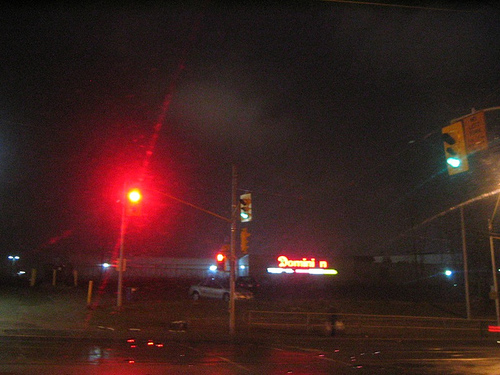
\includegraphics[width=\linewidth]{./figure+object/2015_02610.jpg}
    \caption{Image with ``Car" Class}
    \label{fig:car}
  \end{minipage}%
  \hfill
  \begin{minipage}{.45\textwidth}
    \centering
    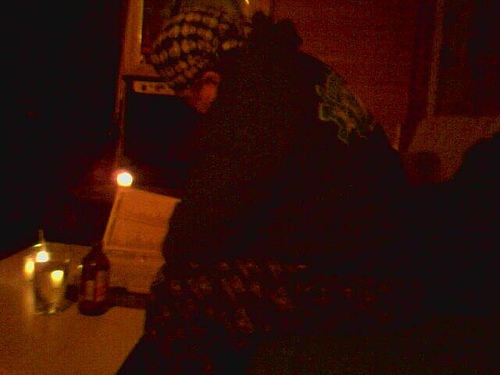
\includegraphics[width=\linewidth]{./figure+object/2015_01439.jpg}
    \caption{``Bottle" and ``People" Class}
    \label{fig:bottle+people}
  \end{minipage}
\end{figure}


In Figure \ref{fig:bottle+people}, the resolution of this image is very low, and the mouth of the bottle and the dark environment next to it are integrated and have no chromatic aberration.

\section{Methods}
\subsection{Annotation Processing and Analysis}
We merged, analyzed, and streamlined the dataset annotations associated with each image. This included calculating the area of objects within the images and designating the largest object in each image as the main label for simplicity and efficiency. Additionally, we developed a custom tool to extract this information, including file names, spatial details, and class types, from each image's accompanying text file. This data was then systematically organized into a spreadsheet format, compatible with the \texttt{Pandas} library for efficient processing and analysis.


\subsection{Image Augmentation}
\paragraph{Resizing and Cropping}: The images were first resized to a \(512 \times 512\) resolution. A dynamic approach was then adopted for cropping, where we modified the scale range of \(0.8\) to \(1.0\) and an aspect ratio range of \(3/4\) to \(4/3\) for image preprocessing, ensuring the cropped images maintained a consistent aspect ratio. The images were finally resized to \(256 \times 256\) to standardize their dimensions.


\paragraph{Random Vertical Flip}: To introduce variation and augment the dataset, we implemented a random vertical flip on the images.


\subsection{Advanced Image Enhancement}
Advanced image enhancement techniques were applied to improve image quality:


\textbf{Contrast Limited Adaptive Histogram Equalization (CLAHE):} Enhances image contrast with a controlled clip limit. We will mainly use this approach.


\begin{figure}[h]
  \centering
  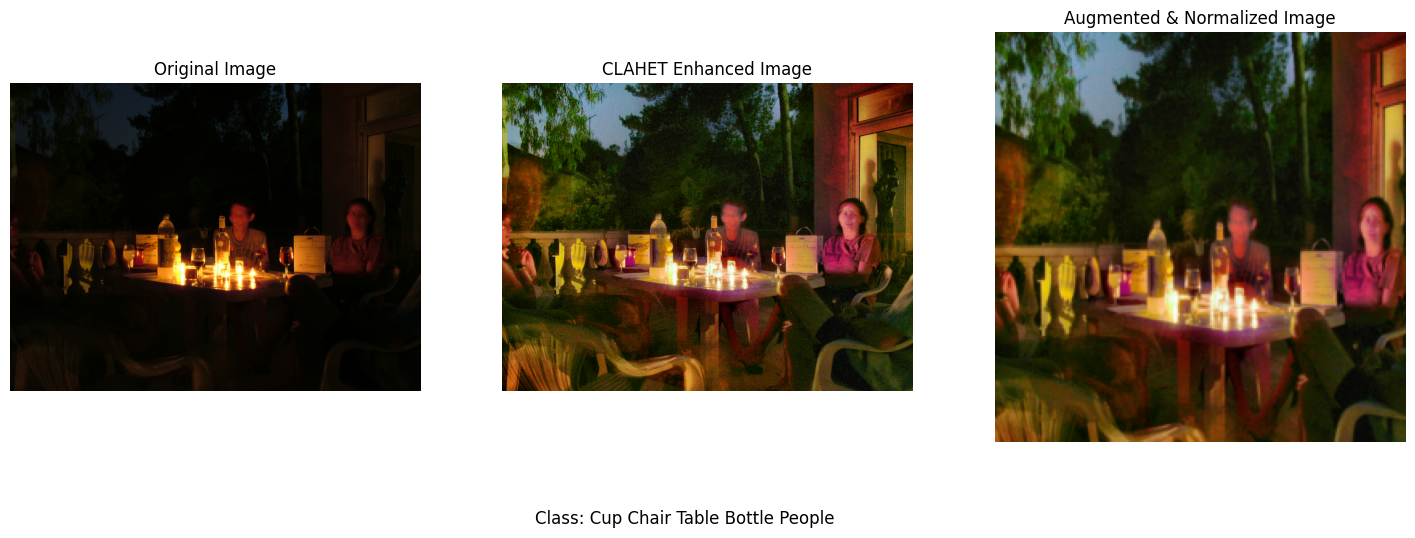
\includegraphics[width=\textwidth]{./figure+object/CLAHET.png}
  \caption{CLAHE}
  \label{fig:clahe}
\end{figure}\hfill


\textbf{Histogram Equalization (HE):} Improves the contrast of the images.


\begin{figure}[h]
  \centering
  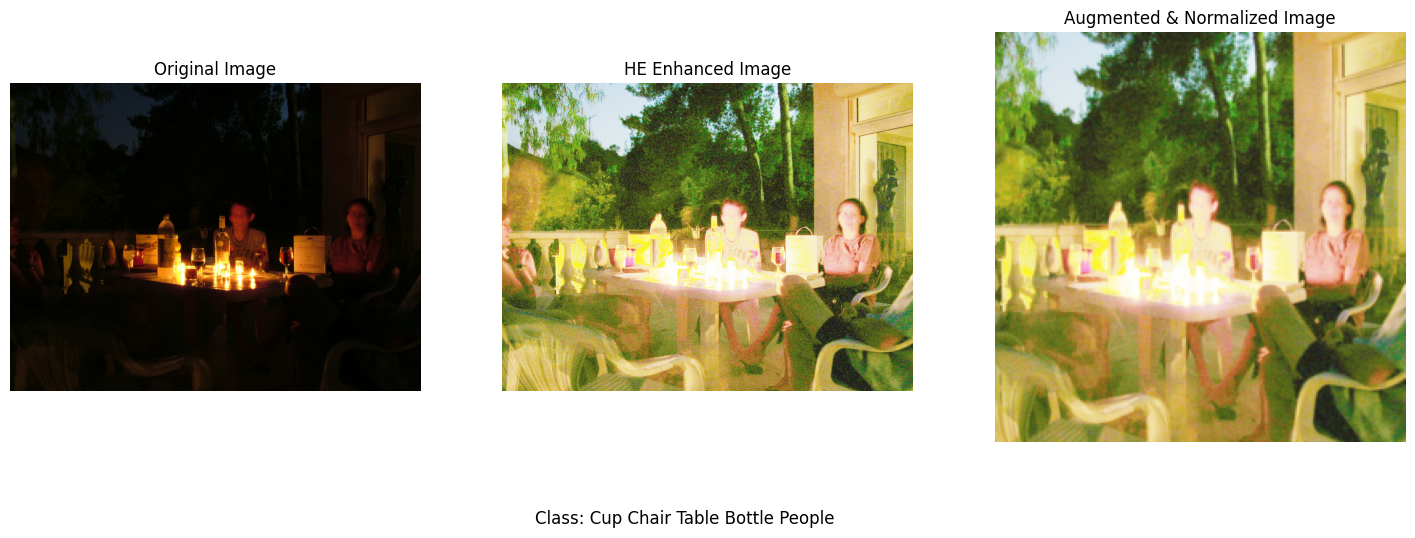
\includegraphics[width=\textwidth]{./figure+object/HE.png}
  \caption{Histogram Equalization}
  \label{fig:he}
\end{figure}\hfill


\textbf{Dynamic Range Adjustment (DRA):} Normalizes the range of pixel intensities.


\begin{figure}[h]
  \centering
  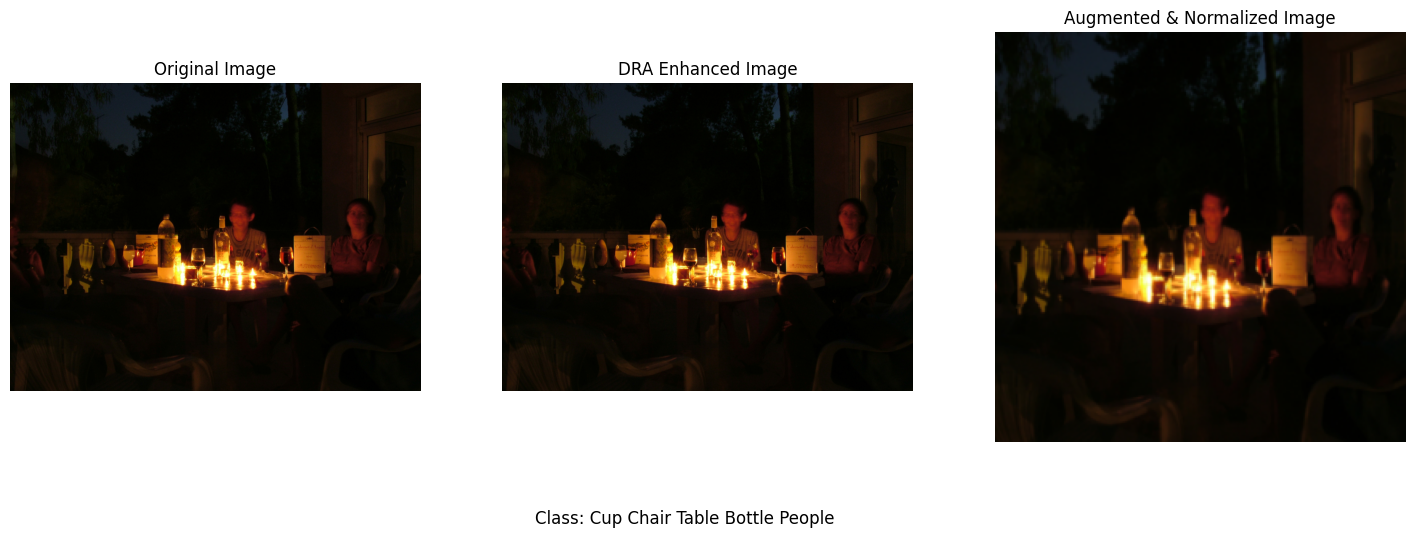
\includegraphics[width=\textwidth]{./figure+object/DRA.png}
  \caption{Histogram Equalization}
  \label{fig:dra}
\end{figure}\hfill


\textbf{Gaussian Blur (GB):} Reduces image noise, focusing on preserving quality.


\begin{figure}[h]
  \centering
  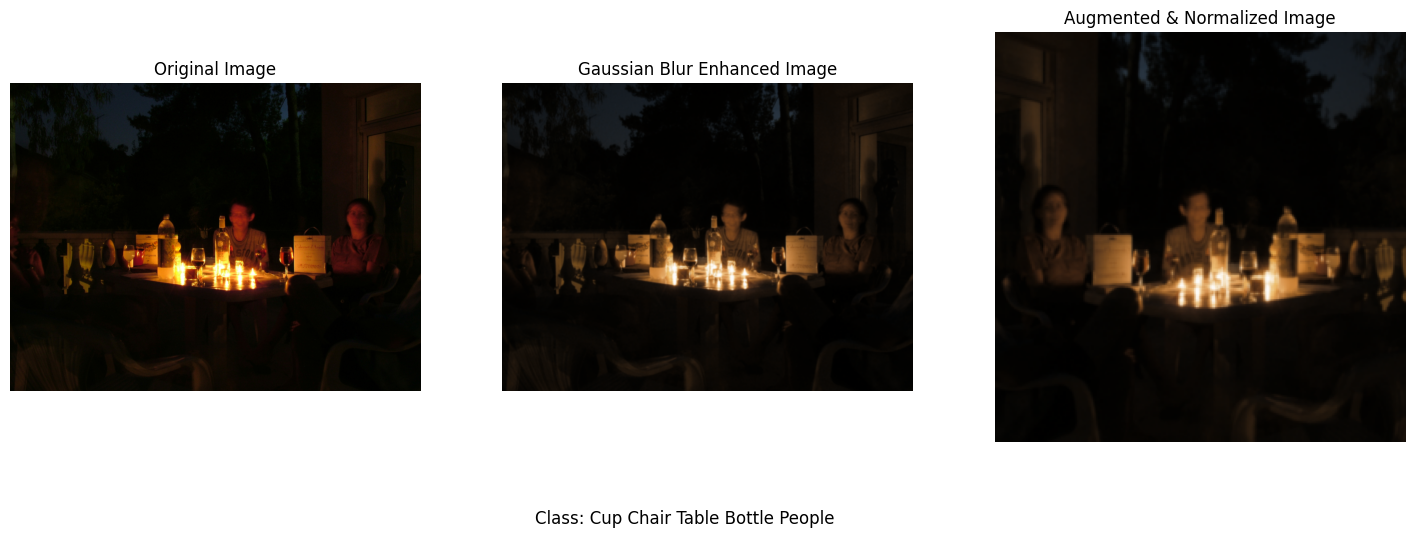
\includegraphics[width=\textwidth]{./figure+object/GB.png}
  \caption{Histogram Equalization}
  \label{fig:gb}
\end{figure}\hfill


\subsection{Transformation Pipeline}
A preprocessing pipeline integrated these methods, designed for flexibility and scalability to incorporate additional techniques as necessary. The advanced image enhancement and augmentation methods were cohesively integrated into a robust preprocessing pipeline, which was designed with flexibility and scalability in mind to accommodate additional techniques and modifications as needed.


\subsection{Normalization}
Two normalization methods were explored in our study: Custom normalization and ImageNet\textsuperscript{\ref{note4}}  normalization. The first approach utilized standard ImageNet\textsuperscript{\ref{note4}}  parameters, while the second involved computing the mean and standard deviation of our images, tailored specifically for the ExDark dataset\textsuperscript{\ref{note1}}. Interestingly, even though our custom normalization was specifically designed for the ExDark dataset\textsuperscript{\ref{note1}}, we observed that the standard ImageNet\textsuperscript{\ref{note4}}  parameters outperformed our method in VGG\textsuperscript{\ref{note2}} and ResNet\textsuperscript{\ref{note3}} models. Conversely, our custom normalization demonstrated superior performance in our specially designed baseline CNN. This finding suggests that the optimal normalization method is dependent on the model architecture and custom dataset.


\subsection{Custom Dataset Preparation}
In processing the annotations, we prioritized the largest object in each image as the primary label, based on its spatial dimensions. This approach was adopted to enhance accuracy and reflect real-world scenarios where the most prominent object is often of the highest relevance.


Our research necessitated creating custom datasets for the effective training and evaluation of various neural network models. We developed specialized datasets for binary (Creature vs. Auto), ternary (People vs. Cat vs. Dog), and multilabel classifications, each tailored to meet the specific requirements of these classification tasks.


\paragraph{Stratified Splitting and Sampling:} We employed stratified sampling to divide the datasets into training and testing sets, ensuring balanced class representation. For the ternary dataset, a WeightedRandomSampler was used to mitigate class imbalance during training. A custom PyTorch dataset class was developed to streamline the loading and transformation of images and labels, integrating effectively with PyTorch's DataLoader.


\paragraph{Binary Classification Dataset:} This dataset was constructed by filtering annotations to include classes relevant for binary classification, such as \textbf{Creatures} (People, Cat, and Dog) and \textbf{Autos} (Car, Bus, Bicycle, and Motorbike). It played a crucial role in training models to distinguish between these broad categories.


\paragraph{Ternary Classification Dataset:} We developed a ternary classification dataset by selecting appropriate classes from the annotations, specifically targeting ``People", ``Cat", and ``Dog". This dataset was designed to refine the classification process for images identified as ``Creature" in the binary classification phase. It enables the models to further categorize a ``Creature" into one of the three more specific categories, enhancing the accuracy and granularity of our classification system.


\paragraph{Multilabel N-ary Classification Dataset:} Designed to handle images with 12 distinct labels, this dataset was vital for training models to simultaneously predict several classes, capturing the overlapping nature of objects in the ExDark dataset\textsuperscript{\ref{note1}}.


\subsection{Models}
Our exploration of neural network models was comprehensive, focusing on three distinct architectures, each adapted for binary, ternary, and multilabel N-ary classification tasks. We chose to investigate a handcrafted CNN, and the well-established VGG19\textsuperscript{\ref{note2}} and ResNet50\textsuperscript{\ref{note3}} models, modifying each to meet the specific demands of the ExDark dataset\textsuperscript{\ref{note1}}'s diverse and complex nature.

\paragraph{Handcrafted CNN:} Our initial model, a custom CNN with three convolutional layers, was specifically developed to align with our dataset. However, we encountered challenges during training, as the model's learning stagnated with a consistent loss around 0.6913, indicating underfitting. This led us to explore more sophisticated architectures.

\paragraph{Modified ResNet50\textsuperscript{\ref{note3}}:} We utilized the ResNet50\textsuperscript{\ref{note3}} architecture, known for its effective training of deep networks through residual learning. The model was initialized with pre-trained weights, and its final fully connected (FC) layer was adapted to accommodate the number of classes in our dataset, enhancing its suitability for our specific classification tasks.

\paragraph{Modified VGG19\textsuperscript{\ref{note2}}:} Our approach with VGG19\textsuperscript{\ref{note2}} involved leveraging its deep and robust feature extraction capabilities. Like ResNet50\textsuperscript{\ref{note3}}, we started with a pre-trained VGG19\textsuperscript{\ref{note2}} model and modified its final FC layer to map to the dataset's class structure, thus tailoring it for our classification requirements.

Each of these models - the custom CNN, modified ResNet50\textsuperscript{\ref{note3}}, or modified VGG19\textsuperscript{\ref{note2}} - was chosen for their unique architectures and learning capabilities. The custom CNN provided a baseline and a deeper understanding of the dataset's complexity. In contrast, the modified versions of VGG19\textsuperscript{\ref{note2}} and ResNet50\textsuperscript{\ref{note3}} brought the advantage of advanced feature extraction and deep learning techniques, which were hypothesized to be more effective for the challenging conditions presented by the ExDark dataset\textsuperscript{\ref{note1}}.

\section{Experiments}
\subsection{Hyper-parameters}
A substantial portion of our research, over 50\%, was devoted to the meticulous process of identifying the most suitable hyper-parameters for our models. This critical aspect proved to be a challenging yet essential part of our study, greatly influencing model performance and accuracy.


\begin{itemize}
  \item \textbf{Learning Rate:} A standard rate of \(1e-5\) was used, with adjustments made for larger models.
  \item \textbf{Optimizer:} The Adam optimizer was employed across all models for its efficiency.
  \item \textbf{Criterion:} Various criteria were used depending on the classification task:
    \begin{itemize}
      \item Binary: CrossEntropyLoss and BCEWithLogitsLoss.
      \item Ternary: CrossEntropyLoss.
      \item Multilabel N-ary: BCEWithLogitsLoss.
    \end{itemize}
  \item \textbf{Sampler:} The WeightedRandomSampler was utilized to address class imbalance, particularly in the ternary classification.
  \item \textbf{Scale and Aspect Ratio:} We maintained a scale range of \(0.8-1.0\) and an aspect ratio range of \(3/4-4/3\) for image preprocessing.
  \item \textbf{Normalization:} Both ImageNet\textsuperscript{\ref{note4}}  parameters and custom RGB mean and standard deviation values were used.
  \item \textbf{Customized CNN Model Parameters:}
    \begin{itemize}
      \item Convolutional layers: 3 layers.
      \item Fully connected layers: 3 layers.
      \item Pooling: MaxPool2d and AdaptiveAvgPool2d.
      \item Activation functions: ReLU, Sigmoid, Softmax.
    \end{itemize}
  \item \textbf{Label Selection Criteria:} The largest object's spatial dimensions were used in each image as the primary label in enhancing classification accuracy.
\end{itemize}


\subsection{Binary Classification}
\paragraph{Model Introduction and Build:} 
Our binary classification study began with a Custom CNN, ResNet50\textsuperscript{\ref{note3}}, and VGG19\textsuperscript{\ref{note2}}. Each model was fine-tuned using BCEWithLogitsLoss, and CrossEntropyLoss was also evaluated for a thorough analysis. The primary objective was to accurately classify images into ``Creature" and ``Auto" categories.

\paragraph{Classification Report and Analysis:}
In our analysis, \textbf{BCEWithLogitsLoss} demonstrated superiority over \textbf{CrossEntropyLoss} in terms of precision, recall, and overall accuracy. The \textbf{Custom CNN} processed data over 20 epochs in 34 minutes, achieving an accuracy of 70.2899\% and a loss of 0.4318. It showed a precision of 0.76 for `Creature' and 0.66 for `Auto', with a higher recall for `Creature`. \textbf{ResNet50\textsuperscript{\ref{note3}}}, in 27 minutes, achieved an accuracy of 93.5818\% with a loss of 0.0179, showing a superior precision of 0.95 for `Creature' and 0.92 for `Auto'. \textbf{VGG19\textsuperscript{\ref{note2}}}, within the same duration, reached an accuracy of 91.92\% and a loss of 0.0074, slightly favoring `Auto', with precision values of 0.93 and 0.91 for `Auto' and `Creature' respectively.

\paragraph{Confusion Matrix Analysis:}
The confusion matrices revealed the effectiveness of BCEWithLogitsLoss, particularly noteworthy in the \textbf{ResNet50\textsuperscript{\ref{note3}}} model, which displayed a balanced classification ability. The \textbf{Custom CNN} accurately identified 333 instances of ``Creature" while misclassifying 107, and correctly classified 346 instances of ``Auto". \textbf{ResNet50\textsuperscript{\ref{note3}}} demonstrated a balanced performance with 478 true positives for ``Creature" and 426 for ``Auto". \textbf{VGG19\textsuperscript{\ref{note2}}} exhibited a slight bias towards ``Creature", with 481 true positives as opposed to 404 for ``Auto".

\begin{figure}[htbp]
  \centering
  \begin{minipage}{.3\textwidth}
    \centering
    \includegraphics[width=\linewidth]{./figure+object/cnn_binary_bce.png}
    \caption{CNN Binary}
    \label{fig:cnn_cm_bin}
  \end{minipage}%
  \hfill
  \begin{minipage}{.3\textwidth}
    \centering
    \includegraphics[width=\linewidth]{./figure+object/resnet_binary_bce.png}
    \caption{ResNet50 Binary}
    \label{fig:resnet_cm_bin}
  \end{minipage}%
  \hfill
  \begin{minipage}{.3\textwidth}
    \centering
    \includegraphics[width=\linewidth]{./figure+object/vgg_binary_bce.png}
    \caption{VGG19 Binary}
    \label{fig:vgg_cm_bin}
  \end{minipage}
\end{figure}


\paragraph{Overall Performance:}
BCEWithLogitsLoss emerged as the superior criterion for binary classification, with ResNet50\textsuperscript{\ref{note3}} slightly leading in terms of precision and accuracy.


\paragraph{Experiences:}
Our exploration into binary classification highlighted the importance of the right loss function choice. While both BCEWithLogitsLoss and CrossEntropyLoss were effective, BCEWithLogitsLoss was chosen for its superior performance, though CrossEntropyLoss's slightly lesser results also provide valuable insights for future applications.


\subsection{Ternary Classification}
\paragraph{Model Introduction and Build:}
Expanding from binary to ternary classification, we focused on distinguishing among ``People", ``Cat", and ``Dog". We utilized a Custom CNN, ResNet50\textsuperscript{\ref{note3}}, and VGG19\textsuperscript{\ref{note2}}, each trained with BCEWithLogitsLoss, to tackle this more nuanced classification task.

\paragraph{Classification Report and Analysis:}
In the ternary classification task, each model exhibited distinct performances. The \textbf{Custom CNN} processed data over 20 epochs, ending with a loss of 0.8354 and an accuracy of 52.8265\%, achieved in 34 minutes. It showed precision scores of 0.67 for ``People", 0.46 for ``Cat", and 0.31 for ``Dog", favoring ``People" more. The \textbf{ResNet50\textsuperscript{\ref{note3}}} model excelled with an accuracy of 92.3977\% and a loss of 0.0560, showing high precision across all classes - 0.98 for ``People", 0.92 for ``Cat", and 0.82 for ``Dog". \textbf{VGG19\textsuperscript{\ref{note2}}}, processing data in the same duration, achieved an accuracy of 90.64\% with a loss of 0.0289. It displayed a high precision for ``People"(0.95) but slightly lower for ``Cat'' and ``Dog" at 0.78 and 0.86.

\paragraph{Confusion Matrix Analysis:}
The confusion matrices provided valuable insights into the classification behavior of each model in the ternary task. The \textbf{Custom CNN}'s matrix showed a tendency to correctly classify ``People" with 178 true positives, but it also had notable misclassifications, as shown in the matrix below. In contrast, the \textbf{ResNet50\textsuperscript{\ref{note3}}} model exhibited excellent balance and high accuracy, with impressive 240 true positives for ``People", and true positives for ``Cat" (123) and ``Dog" (111). Similarly, \textbf{VGG19\textsuperscript{\ref{note2}}} demonstrated its proficiency, especially in classifying ``People" with 244 true positives, and performed well for ``Cat" (118 true positives) and ``Dog" (89 true positives), confirming its effectiveness in this challenging classification environment.

\begin{figure}[htbp]
  \centering
  \begin{minipage}{.3\textwidth}
    \centering
    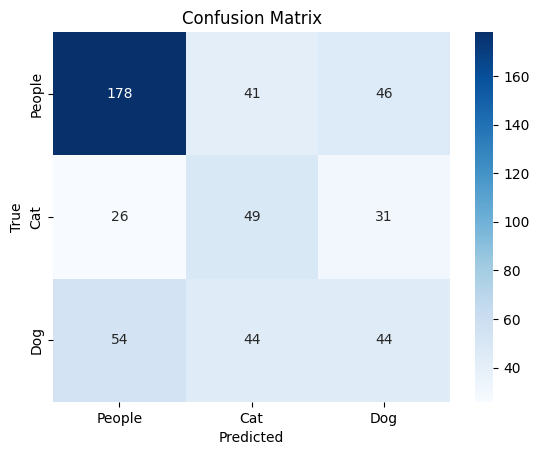
\includegraphics[width=\linewidth]{./figure+object/CNN_ternary_BCE.png}
    \caption{CNN Ternary}
    \label{fig:cnn_cm_ter}
  \end{minipage}%
  \hfill
  \begin{minipage}{.3\textwidth}
    \centering
    \includegraphics[width=\linewidth]{./figure+object/resnet_ternary_BCE.png}
    \caption{ResNet50 Ternary}
    \label{fig:resnet_cm_ter}
  \end{minipage}%
  \hfill
  \begin{minipage}{.3\textwidth}
    \centering
    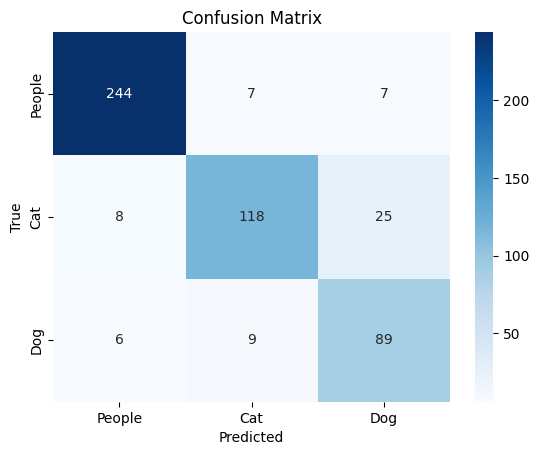
\includegraphics[width=\linewidth]{./figure+object/VGG_ternary_BCE.png}
    \caption{VGG19 Ternary}
    \label{fig:vgg_cm_ter}
  \end{minipage}
\end{figure}


\paragraph{Overall Performance:}
ResNet50\textsuperscript{\ref{note3}} and VGG19\textsuperscript{\ref{note2}} exhibited robustness in ternary classification, efficiently managing the task's complexity. The Custom CNN, while less accurate, provided valuable insights into the dynamics of classifying these closely related categories.

\paragraph{Experiences:}
The ternary classification phase underscored the challenge of dataset imbalance. The implementation of a WeightedRandomSampler was critical in achieving balanced exposure across classes, particularly benefiting the less represented ``Cat" and ``Dog" classes. This phase reinforced the importance of strategic sampling and advanced modeling techniques in complex classification tasks, and highlighted the necessity for refined tuning and richer datasets in multiclass machine learning scenarios.


\subsection{Multilabel N-ary Classification}
\paragraph{Model Introduction and Build:}
We ventured into the challenging realm of multilabel N-ary (12 classes) classification, employing our Custom CNN, ResNet50\textsuperscript{\ref{note3}}, and VGG19\textsuperscript{\ref{note2}} with BCEWithLogitsLoss. This phase marked a significant leap in complexity, requiring our models to discern multiple classes within a single image.

\paragraph{Classification Report:}
The \textbf{Custom CNN} struggled, managing only an 8.2154\% accuracy over 20 epochs and 66 minutes of training. The model's limitations were evident in its inconsistent precision and recall across various classes, with notable struggles in classifying ``Bicycle" and ``Bottle". Conversely, \textbf{ResNet50\textsuperscript{\ref{note3}}} demonstrated a robust performance, achieving a significant accuracy of 60.1494\% in 51 minutes. It showed high precision in most classes, particularly excelling with ``Boat" and ``Dog". \textbf{VGG19\textsuperscript{\ref{note2}}} also performed commendably, reaching 54.8540\% accuracy in 55 minutes. While slightly behind ResNet50\textsuperscript{\ref{note3}}, VGG19\textsuperscript{\ref{note2}} displayed substantial precision and recall, marking it as a capable model for multilabel classification tasks.

\paragraph{Confusion Matrix Analysis:}
\textbf{Custom CNN's} revealed significant misclassifications, especially in complex categories. For instance, ``Bicycle" saw only 18 true positives against 132 negatives, highlighting the model's difficulty with finer-grained classification. Classes with more nuanced features, like ``Bottle" and ``Cup", had true positives of only 0 and 47 respectively, suggesting that the CNN model struggled to distinguish between similar object categories. \textbf{ResNet50\textsuperscript{\ref{note3}}} demonstrated a robust ability to correctly identify multiple labels. Notable performances include ``Bicycle" and ``Bus" with high true positive rates of 1307 and 1356, respectively. This model showed a high level of precision across most classes, although some, like ``Motorbike" and ``Table", still presented room for improvement with lower true positive rates. \textbf{VGG19\textsuperscript{\ref{note2}}}, then indicated a competent classification capability with a relatively even distribution of true positives across classes. However, there were instances of confusion, such as between ``Dog" and ``Motorbike", where the true positive rates were not as high as expected. This suggests that while VGG19\textsuperscript{\ref{note2}} was adept at multilabel classification, certain classes could benefit from further model refinement to reduce misclassification.

\begin{figure}[htbp]
  \centering
  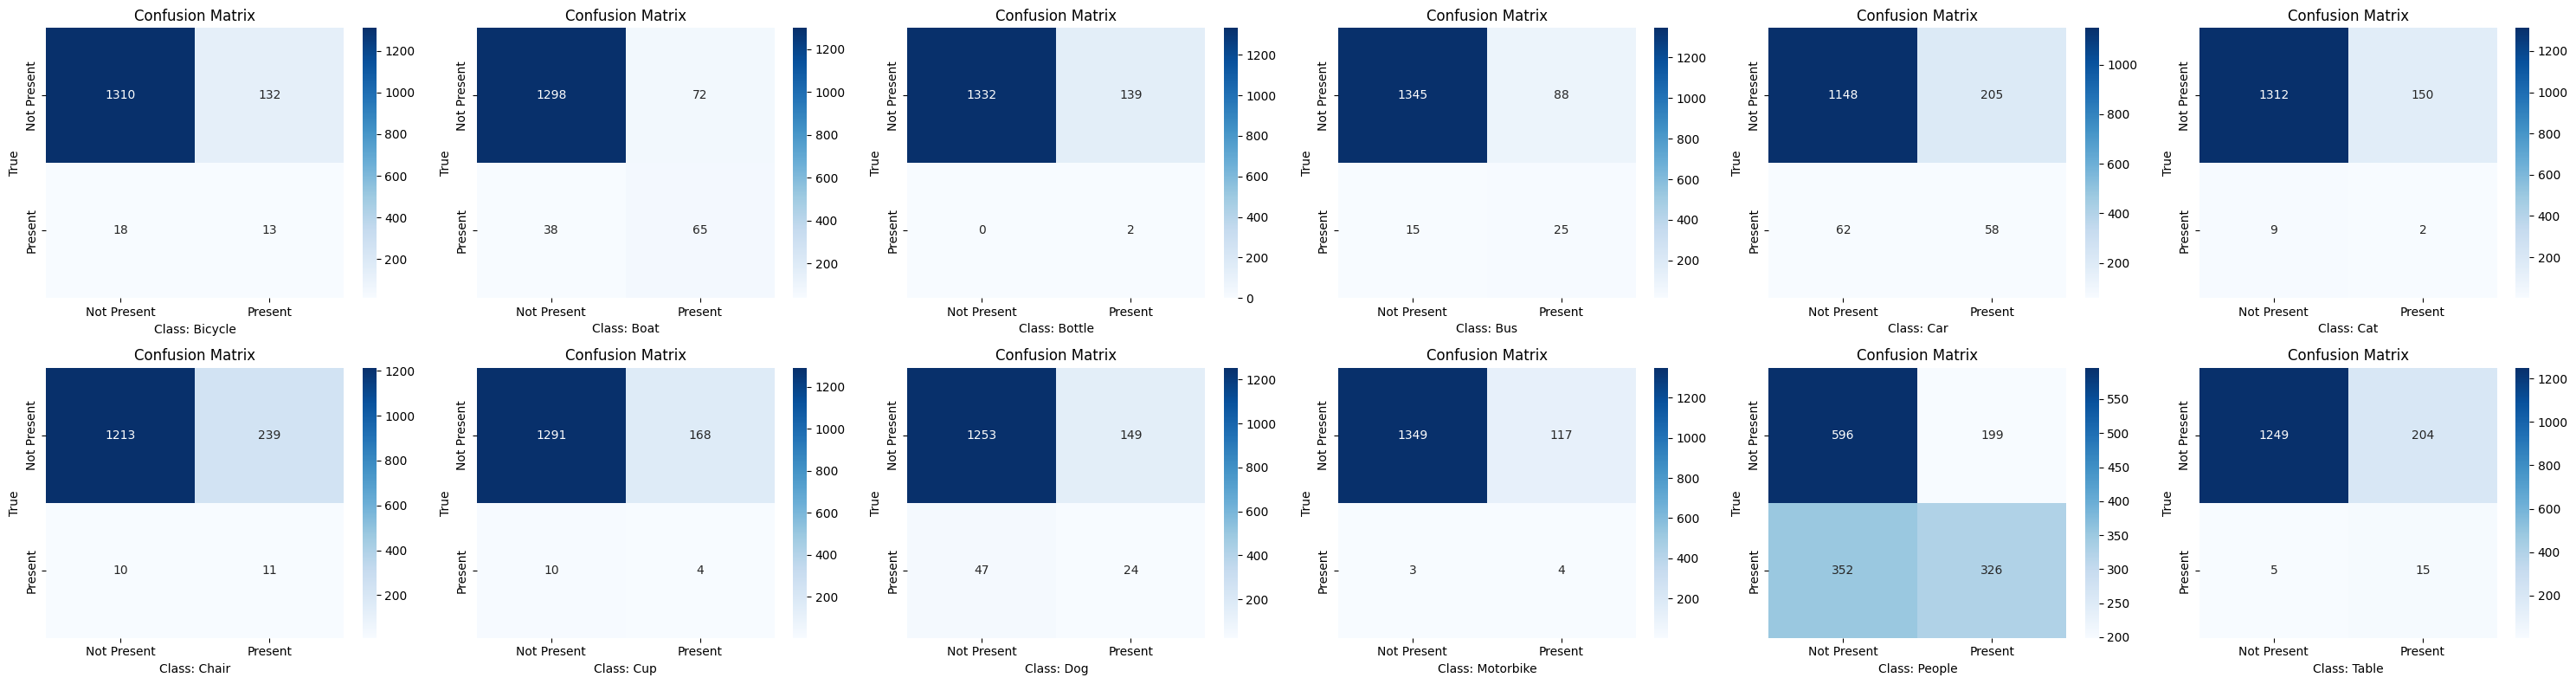
\includegraphics[width=1.0\textwidth]{./figure+object/CNN_labels_BCE.png}
  \caption{CNN Multilabel N-ary Confusion Matrix}
  \label{fig:cnn_cm_mul}
\end{figure}

\begin{figure}[htbp]
  \centering
  \includegraphics[width=1.0\textwidth]{./figure+object/resnet_labels_BCE.png}
  \caption{ResNet50 Multilabel N-ary Confusion Matrix}
  \label{fig:resnet_cm_mul}
\end{figure}


\begin{figure}[htbp]
  \centering
  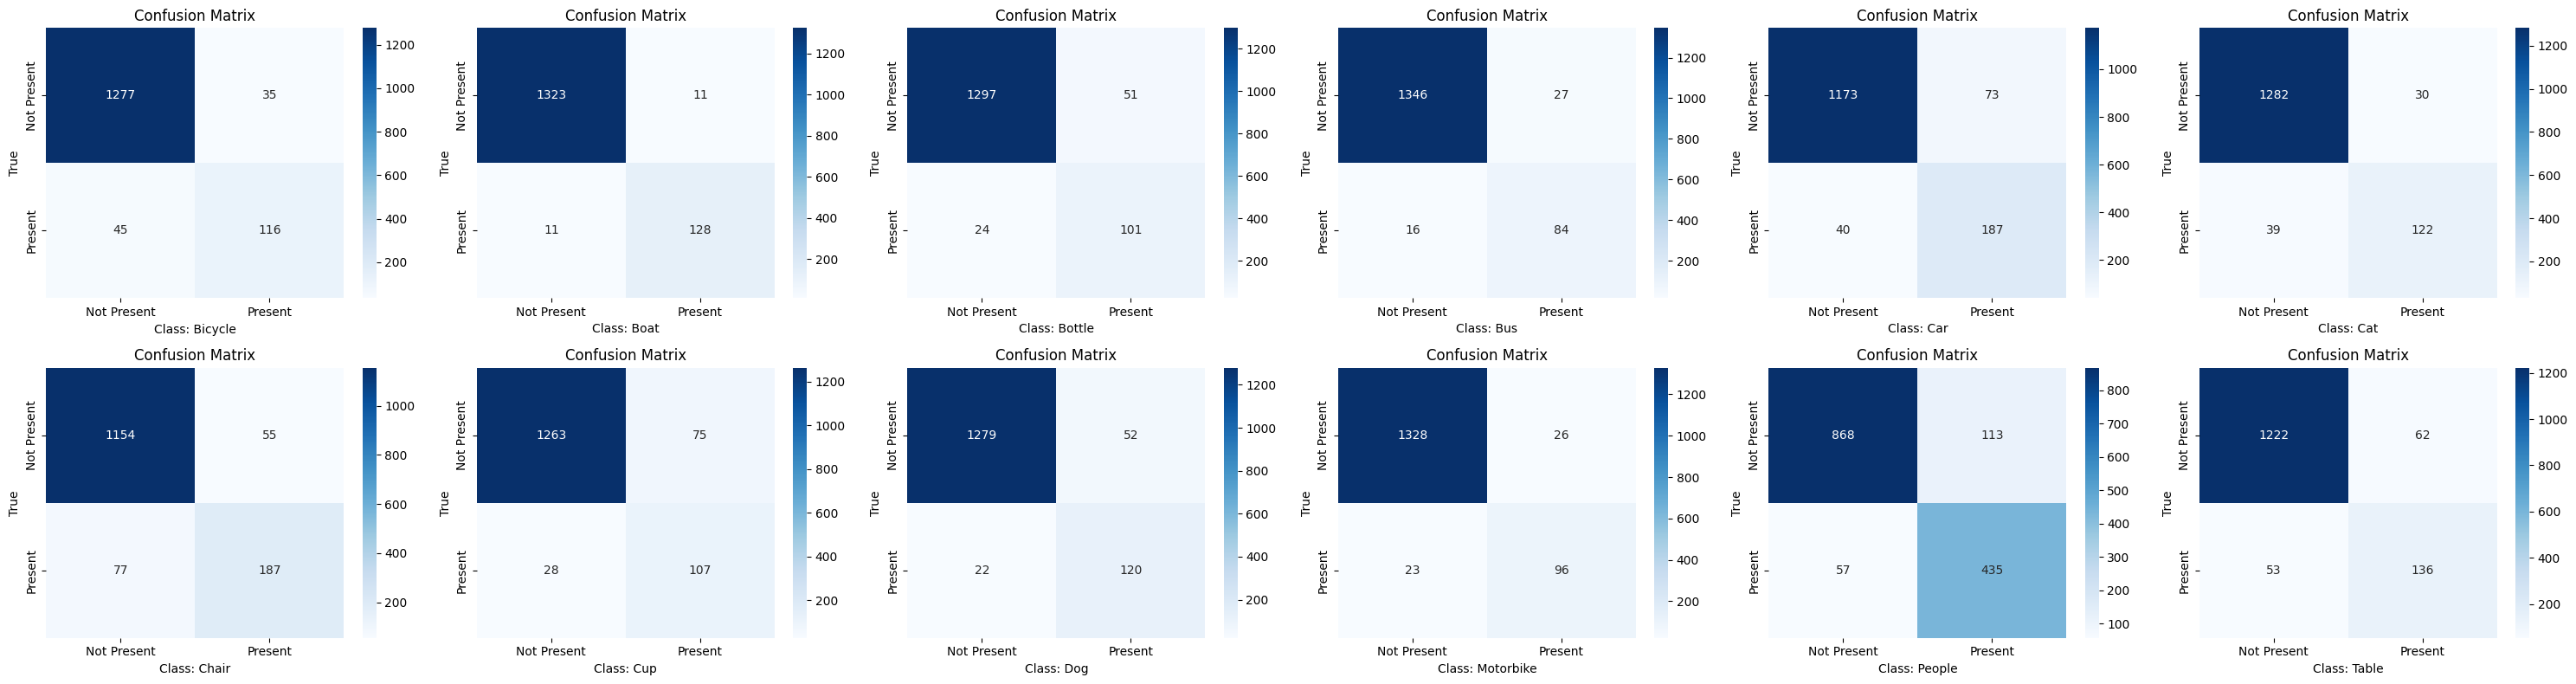
\includegraphics[width=1.0\textwidth]{./figure+object/VGG_labels_BCE.png}
  \caption{VGG19 Multilabel N-ary Confusion Matrix}
  \label{fig:vgg_cm_mul}
\end{figure}

\paragraph{Overall Performance:}
ResNet50\textsuperscript{\ref{note3}} and VGG19\textsuperscript{\ref{note2}} showcased their capabilities in the multilabel scenario, with ResNet50\textsuperscript{\ref{note3}} slightly ahead in performance compared to VGG19\textsuperscript{\ref{note2}}. The Custom CNN, in contrast, was less effective in this complex classification task.

\paragraph{Experiences:}
The multilabel classification phase of our research illuminated crucial challenges, notably the imbalance among different classes. We effectively addressed this using a WeightedRandomSampler, ensuring equitable representation in model training. However, a noticeable discrepancy emerged between high precision/recall for individual classes and lower overall accuracy. This underscored the complexity of the images and the necessity of sophisticated modeling techniques. The phase affirmed the need for advanced model architectures in multilabel tasks, emphasizing the significance of considering data distribution and characteristics for effective machine learning strategies.


\subsection{Discussion}
This study embarked on a comprehensive exploration of image classification across binary, ternary, and multilabel N-ary tasks, employing a custom CNN alongside established architectures such as ResNet50\textsuperscript{\ref{note3}} and VGG19\textsuperscript{\ref{note2}}. Notably, the models were benchmarked against a backdrop of rigorous hyperparameter tuning, which constituted over half of the research effort, underscoring its criticality in optimizing model performance.


\subsubsection{Binary Classification}
The binary classification task illuminated the distinct efficacies of different loss functions. Our custom CNN, though not as swift or accurate as its more sophisticated counterparts, nonetheless contributed valuable insights, particularly in the distinction between ``Creature" and ``Auto" classes. It was observed that the precision and recall metrics varied significantly between the classes, with a higher recall noted for ``Creature". This could be attributed to the innate model biases or the data distribution within the training set.


ResNet50\textsuperscript{\ref{note3}} emerged as the front-runner, achieving a commendable balance between precision and recall across both classes. VGG19\textsuperscript{\ref{note2}}'s performance was closely aligned with ResNet50\textsuperscript{\ref{note3}}'s, albeit with a slight bias towards the ``Creature" class. These results showcase the potential of advanced architectures in handling binary classifications with high accuracy, provided that the model is well-tuned.


\subsubsection{Ternary Classification}
Ternary classification expanded the challenge by introducing an additional class, thereby increasing the complexity of the task. The models were put to the test, with ResNet50\textsuperscript{\ref{note3}} once again demonstrating its robustness, closely followed by VGG19\textsuperscript{\ref{note2}}. The custom CNN struggled in this scenario, emphasizing the need for more complex model architectures when dealing with an increased number of classes. The WeightedRandomSampler played a pivotal role in mitigating the class imbalance, which was particularly pronounced in this classification scheme.


\subsubsection{Multilabel N-ary Classification}
Venturing into the realm of multilabel N-ary classification, the study highlighted the intricate nature of identifying multiple objects within a single image. The overall performance saw ResNet50\textsuperscript{\ref{note3}} leading, with VGG19\textsuperscript{\ref{note2}} close behind. The custom CNN faced challenges, reflecting the heightened complexity of the task at hand. Precision and recall metrics varied widely across classes, with some like ``Bottle" achieving high precision but low recall, indicating a model reluctant to predict that class unless very certain.


The ResNet50\textsuperscript{\ref{note3}} model demonstrated commendable performance in discerning ``Boat" and ``Dog" classes, while the custom CNN exhibited limitations in differentiating finer-grained categories.


\subsubsection{Implications and Future Work}
Our findings have significant implications for the development of image classification systems. It becomes evident that while custom models may offer a starting point, the sophistication offered by advanced pre-trained architectures like ResNet50\textsuperscript{\ref{note3}} and VGG19\textsuperscript{\ref{note2}} is indispensable for higher accuracy and balanced precision-recall metrics. Moreover, the use of weighted sampling to address class imbalance proved crucial, suggesting that future research should continue to focus on methods for equitable class representation.


In terms of future work, exploring additional data augmentation strategies, further hyperparameter optimization, and the integration of more complex models could yield improvements in classification tasks. Moreover, diving into the intricacies of dataset composition and investigating the potential of ensemble methods may provide pathways to enhance model robustness and accuracy


\section{Conclusion}
Our study marks a significant advancement in the field of image classification under challenging conditions, demonstrating the effectiveness of our model pipeline. The research opens new avenues for innovative applications and integrations with other advanced machine-learning solutions.


Particularly noteworthy is our approach's impact on ternary classification, tailored for specific tasks. This success sets the stage for further exploration and application in fields requiring nuanced image interpretation, such as autonomous systems and advanced surveillance.


The transition from binary to multilabel N-ary classification not only deepened our understanding of the field's challenges but also established a foundation for future machine-learning explorations. Our model pipeline's adaptability and effectiveness highlight its potential for real-world applications, promising significant contributions to areas where precise classification is crucial.


In conclusion, this study paves the way for innovative applications and integrations in Deep Learning, reflecting our model pipeline's potential in areas demanding accurate and nuanced image interpretation.


\newpage
\bibliography{iclr2024_conference}
\bibliographystyle{iclr2024_conference}

\end{document}
